\section{Metodyka Scrum} \label{scrum}

Jednym z~podstawowych celów pracy inżynierskiej jest przedstawienie (prezentacja) wykorzystanych w~niej technologii, narzędzi, metod itp. Ze~względu na~użycie podczas pisania mojej pracy metodologii Scrum (używanej powszechnie w~małych i~średnich firmach -- nie tylko programistycznych) zamierzam opisać tę~metodologię i~zaprezentować w~prosty sposób jej przebieg.


Scrum \cite{scrumalliance} (z~ang. scrum -- przepychanka, młyn) jest jedną z~wielu pochodnych metodyki programowania zwinnego \cite{agile1} (z~ang. agile programming).

\subsection{Programowanie zwinne} \label{scrum.agile}

Programowanie zwinne jest popularną metodą pracy w~wielu firmach parających się programowaniem. Dla wyjaśnienia czym tak naprawdę jest wystarczy nam odczytać definicję z~Wikipedii \cite{agile2}:

\begin{quote}
Programowanie zwinne (z~ang. Agile software development) -- grupa metodyk wytwarzania oprogramowania opartego o~programowanie iteracyjne (model przyrostowy). Wymagania oraz~rozwiązania ewolu\-ują przy współpracy samozarządzalnych zespołów, których celem jest przeprowadzanie procesów wytwarzania oprogramowania. Pojęcie zwinnego programowania zostało zaproponowane w 2001 w~Agile Manifesto\footnote{Patrz: \url{agilemanifesto.org/principles.html}}.


Generalnie metodyka oparta jest o~zdyscyplinowane zarządzanie projektem, które zakłada częste inspekcje wymagań i rozwiązań wraz z~procesami adaptacji (zarówno specyfikacji jak i~oprogramowania). Metodyka ta~najczęściej znajduje zastosowanie w~małych zespołach programistycznych, w~których nie występuje problem komunikacji, przez co~nie trzeba tworzyć rozbudowanej dokumentacji kodu. Kolejne etapy wytwarzania oprogramowania zamknięte są~w~iteracjach, w~których za~każdym razem przeprowadza się testowanie wytworzonego kodu, zebranie wymagań, planowanie rozwiązań itd. Metoda nastawiona jest na~szybkie wytwarzanie oprogramowania wysokiej jakości.


Metoda nastawiona jest na~bezpośrednią komunikację pomiędzy członkami zespołu, minimalizując potrzebę tworzenia dokumentacji. Jeśli członkowie zespołu są~w~różnych lokalizacjach, to~planuje się codzienne kontakty za~pośrednictwem dostępnych kanałów komunikacji (wideokonferencja, e-mail itp.).
\end{quote}

Więcej informacji można znaleźć na~stronie \url{www.agileprogramming.org} \cite{agile1}.

\subsection{Scrum} \label{scrum.scrum}

Omówię tu~po~krótce metodykę Scrum wykorzystaną podczas realizacji założeń części praktycznej pracy. Metodyka Scrum opiera się na~ścisłych iteracjach, w~których realizowane są~założenia projektowe. Każda iteracja zaczyna się tzw. Sprint~Meeting'iem (z~ang. Sprint meeting -- ,,spotkanie w~biegu'')\footnote{Więcej na~temat metodyki Scrum można znaleźć na~stronie \url{www.scrumalliance.org}}.

\begin{figure}[!t]
\centering
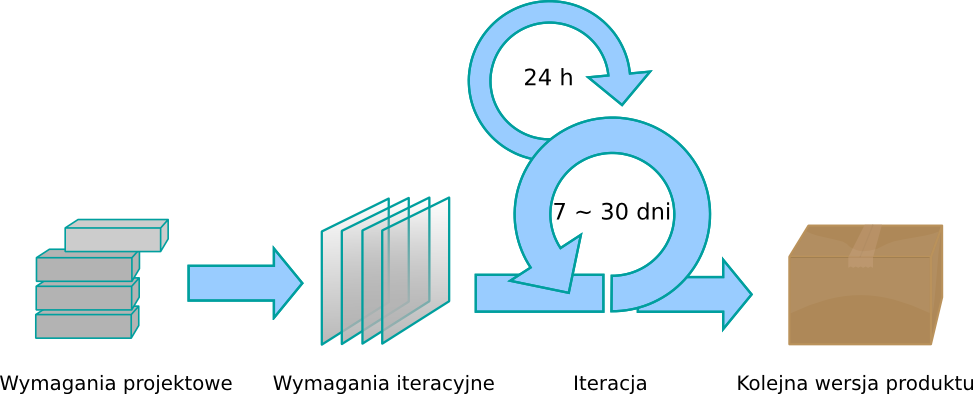
\includegraphics[width=\textwidth]{obrazki/scrum.png}
\caption{Schemat pracy w~kolejnych iteracjach metodyki Scrum (opracowane na~podstawie: \url{http://effectiveagiledev.com/Portals/0/800px-Scrum\_process\_svg.png}).}
\label{fig.rysunek.scrum}
\end{figure}

\subsubsection{Definicje pojęć dla metodyki Scrum} \label{scrum.definicje}

\begin{definition}[Deweloper]
Deweloperem (z~ang. developer -- konstruktor, inwestor) nazywamy osobę bądź firmę\footnote{tu: osobę}, która zaangażowana jest w~realizację czynności związanych z~procesem wytwarzania oprogramowania. Zwykle deweloperem nazywamy członka zespołu projektowego -- programistę.
\end{definition}

\begin{definition}[Iteracja]
Iteracją nazywamy cykl w~procesie wytwarzania oprogramowania, który zamknięty zostaje poprzez zrealizowanie pewnego celu.
\end{definition}

\begin{definition}[Ticket]
Zadania przydzielone zespołowi projektowemu określamy mianem ticketu. Ticket (z~ang. ticket -- bilet) określa jakie obowiązki zostały narzucone na~poszczególnych deweloperów. Jest zwykle odzwierciedleniem żądań i~zaleceń od~klienta.
\end{definition}

\subsubsection{Role} \label{scrum.role}

Główne role jakie można wymienić w~zespole Scrum to:

\begin{enumerate}
  \item Zespół programistyczny (z~ang. The Team) -- wykonawcy projektu, deweloperzy w~liczbie do~9 osób. Do ich obowiązków należy ocena trudności zadań -- ticketów -- realizujących założenia projektowe, realizacja tych zadań oraz~zgłaszanie błędów, trudności itp.~zaistniałych w~projekcie.
  \item Właściciel projektu (z~ang. Product Owner) -- jest to~osoba, firma, grupa itp.~będąca zleceniodawcą (klientem) zatrudniającym zespół programistyczny do~zrealizowania projektu. Zasadniczą rolą właściciela projektu jest przedstawianie założeń, wymagań co~do~projektu, rewizja wykonanych zadań tegoż zespołu oraz~konsultowanie zmian. Gdy właścicielem projektu jest jakaś większa jednostka (firma, spółka, grupa itp.) wtedy wyznaczany jest reprezentant odpowiedzialny za~wyżej wymienione czynności.
  \item Mistrz młyna (z~ang. Scrum Master) -- osoba odpowiedzialna za~komunikację pomiędzy zespołem programistycznym a~właścicielem projektu. Do~jej obowiązków należy przede wszystkim: ustalanie sprint meeting'ów, zgłaszanie intencji zespołu programistycznego, wysyłanie powiadomień o~zmianach w~założeniach itp.
\end{enumerate}

\subsubsection{Rozpoczęcie pracy w~Scrum} \label{scrum.poczatki}

Zanim zostanie otworzona pierwsza iteracja -- sprint -- należy dokładnie przemyśleć i~omówić możliwości grupy projektowej oraz~skonfrontować je~z~wymaganiami klienta. W~tym celu organizowane jest spotkanie inicjujące pracę nad projektem. Na~takim spotkaniu powinny zostać omówione następujące kwestie:

\begin{enumerate}
  \item Omówienie metody pracy z~klientem -- klient powinien wiedzieć jak pracuje zespół  czego może się po~nim spodziewać.
  \item Prezentacja założeń projektowych -- tu~zespół programistyczny dowiaduje się jakie są~postawione wobec niego oczekiwania.
  \item Rewizja założeń projektowych -- zespół programistyczny ma~tu~szansę wypowiedzieć się na~temat kolejnych założeń -- związanych z~nimi trudności, konfrontacja z~umiejętnościami (czego trzeba się ,,douczyć'' a~co~jest zagwarantowane poprzez doświadczenie zespołu).
  \item Wycena projektu oraz~ustalenie licencji jego użytkowania.
\end{enumerate}

Po~omówieniu tych zagadnień klient może zdecydować, czy taki sposób pracy mu~odpowiada. W tym momencie jest w~stanie oszacować jak długo będzie współpracował nad projektem z~tą~grupą projektową, a~co~za~tym idzie -- jaką ilość pieniędzy może przeznaczyć w~poszczególnych etapach tworzenia projektu.

\subsubsection{Sprint meeting} \label{scrum.sprintmeeting}

Sprint meeting zamyka jedną iterację i~rozpoczyna następną. Podczas sprint meeting'u realizowane są zatem: sprawdzenie poprawności wykonanych zadań z~poprzedniej iteracji oraz przedyskutowanie planu pracy w następnej iteracji. Pozwala to klientowi na~pełną kontrolę nad procesem wytwarzania projektu. Do~najważniejszych kwestii omawianych na~sprint meeting'u należą:

\begin{enumerate}
  \item Sprawdzenie stanu wykonanych zadań -- jeśli zadania zostały dostarczone klientowi jako wykonane, to~klient może je~zweryfikować pod względem ich poprawności. Każde takie zadanie może zostać zaakceptowane (wtedy oznaczone zostaje jako wykonane) bądź nie (Zadanie odrzucone wymaga poprawki -- klient może zdecydować, co~powinno być w~tej sytuacji wykonane. Jeżeli klient ma~wystarczająco funduszy na~wykonanie poprawek wtedy może zlecić poprawkę, jeśli nie, to~zadanie może zostać ,,zamrożone'' i~czekać na~pieniądze potrzebne do~jego realizacji. Oczywiście klient może także zaniechać realizacji zadania.).
  \item Określenie wymagań projektowych -- klient wymienia swoje oczekiwania względem projektu. Wymagania te~zostają skonfrontowane z~możliwościami zespołu programistycznego (,,tego nie da~się zrobić'', ,,to~jest za~trudne'', ,,to~wymaga lepszego sprzętu'', ,,realizacja tego zadania zajmie \ldots'', ,,koszta tego zadania wyniosą około \ldots'', albo: ,,to~jest proste'', ,,znamy się na~tym'' itp.). Zwykle zaistniałe trudności w~realizacji zadań kończą się kompromisem. Po~określeniu możliwości realizacji wymagań tworzone są~zadania.
  \item Określenie zadań dla grupy projektowej -- po~,,wycenie'' możliwości deweloperów względem wymagań tworzone są~zadania. Zwykle rozbija się je~na~prostsze, wymagające mniej czasu (według zasady ,,dziel i~zdobywaj'') -- uzyskuje się wtedy płynność w~realizacji zadań, a~praca nad konkretnym wymaganiem podzielona jest pomiędzy członkami zespołu.
  \item Przydzielenie zadań -- klient po~określeniu i~sprecyzowaniu zadań określa ich priorytet. Niektóre zadania są~ważniejsze -- te~oznaczane są~jako zadania przypisane nadchodzącej iteracji -- nad tymi zadaniami grupa projektowa będzie w~najbliższym czasie pracować. Zadania te~zostają następnie wybierane przez konkretnych deweloperów jako te, które będą przez nich realizowane. Jeżeli po~zakończonej iteracji zostaną zadania nie wykonane przez nikogo oznacza to, że~grupa nie nadąża z~tempem pracy narzuconym przez klienta.
  \item Ustalenie ,,dostępności'' deweloperów w~najbliższej iteracji. Członkowie zespołu mogą z~różnych powodów nie móc pracować w~pewnym okresie czasu. Z~tego względu pod koniec sprint meeting'u należy ustalić ile godzin pracy każdy deweloper może przeznaczyć na~najbliższą iterację. Pozwala to~określić ,,siłę'' zespołu oraz~długość iteracji. W~szczególnych przypadkach iteracje mogą zostać przeniesione bądź zawieszone ,,do~odwołania''.
\end{enumerate}

\subsection{Narzędzia Scrum} \label{scrum.narzedzia}

Narzędzi, które wspomagają pracę w~metodyce Scrum jest wiele. Przykładem mogą być tzw. Issue Tracker'y -- środowiska do~zarządzania ticketami. Dobrym przykładem takiego Issue Trackera jest PivotalTracker\footnote{\url{www.pivotaltracker.com}}. Pozwala on~na~kontrolowanie zadaniami poprzez oznaczanie ich jako wykonanych, bieżących itp. Przykładowe zastosowanie tego narzędzia w~pracy nad projektem przedstawia rysunek \ref{fig.rysunek.pivotal}.

\begin{figure}[!t]
\centering
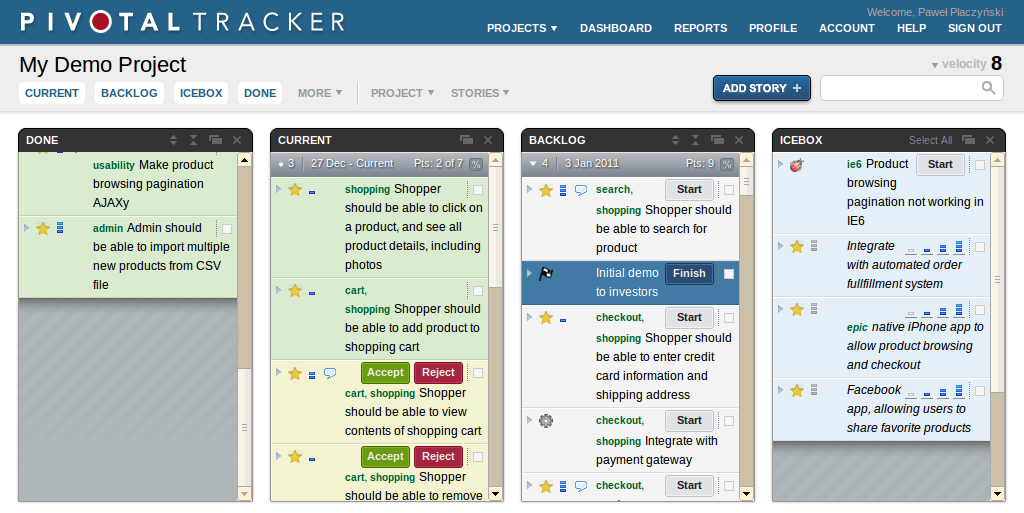
\includegraphics[width=\textwidth]{obrazki/pivotal.png}
\caption{Zastosowanie narzędzia PivotalTracker w~pracy nad projektem (źródło: \url{www.pivotaltracker.com}).}
\label{fig.rysunek.pivotal}
\end{figure}

Innym przykładem narzędzia wspomagającego pracę w~projekcie Scrum są~testy jednostkowe i~funkcjonalne aplikacji (patrz rozdział \ref{dokumentacja.testy}). Służą one tutaj przede wszystkim rewizji zaimplementowanej funkcjonalności a zatem sprawdzeniu poprawności wykonania zadania. Testy takie są~zatem udokumentowaniem wykonanej pracy przez dewelopera.
